%%%% compile with
%%% latexmk -auxdir=aux/ main.tex
\documentclass{irdbeamer}
\usepackage{tikz}
\usepackage{pgfplots}
\usepackage{animate}

\title{Decision trees and Random Forests}
\subtitle{AI for ecologists}
\author[Paul Tresson]{Paul Tresson}
\date{20/05/25} % or whatever the date you are presenting in is
% \institute[Institut de Recherche pour le Développement]{UMR AMAP}

%\copyrightnotice{Published by Institut de Recherche pour le Développement, with permission}

% %% to add a background image for the title slide, uncomment here
% \usebackgroundtemplate{
%   \tikz[overlay, remember picture] \node[at=(current page.center)] {
%     \includegraphics[width=\paperwidth,height=\paperheight]{example-image-a}
%   };
% }

\usepackage[
    backend=biber,
    style=authoryear-comp,
    maxcitenames=2, % max 2 authors before switching to et al.
    maxbibnames=4,
    uniquelist=false, % stays et al. when almost the same authors
    uniquename=false, % dose not bother when first name not written the same way everywhere
    date=year, % month does not appear in bibliography
    natbib=true, % use natbib synthax
    url=false, % remove url
    eprint=false % remove eprint
]{biblatex}

\addbibresource{refs.bib}

\let\oldcite=\cite                                                              
\renewcommand{\cite}[1]{\textcolor[rgb]{.5,.5,.7}{\oldcite{#1}}}
\let\oldcitep=\citep                                                              
\renewcommand{\citep}[1]{\textcolor[rgb]{.5,.5,.7}{\oldcitep{#1}}}

\begin{document}

\addlogo{logos/IRD_banner.png}
\addlogo{logos/AMAP_banner.png}
\addlogo{logos/CESAB.jpg}
\maketitle

\usebackgroundtemplate{}

\section{Introduction}

\begin{frame}{Motivation}
\begin{columns}
    \begin{column}[t]{0.5\textwidth}
\centering
    \includegraphics<1>[width=\textwidth]{./figs/schemas/motivation1.png}%
    \includegraphics<2->[width=\textwidth]{./figs/schemas/motivation2.png}%
\end{column}
    \begin{column}[t]{0.5\textwidth}
\centering
    \includegraphics<3>[width=\textwidth]{./figs/schemas/motivation-tree.png}%
\end{column}
\end{columns}
\end{frame}


\section{Decision Trees}

\begin{frame}{Simple example}
\begin{columns}
    \begin{column}{0.5\textwidth}
\centering
{\small
\begin{tabular}{llc|r}
    \toprule
    Disturbance & Habitat & Avg. temp. & Presence \\
    \midrule
    Yes & Shrubs    & 10 & 0 \\
    Yes & Forests   & 12 & 0 \\
    No  & Shrubs    & 18 & 1 \\
    No  & Shrubs    & 25 & 1 \\
    Yes & Shrubs    & 28 & 1 \\
    Yes & Forests   & 30 & 0 \\
    No  & Forests   & 33 & 0 \\
    \bottomrule
\end{tabular}
        }
    \end{column}
    \begin{column}{0.5\textwidth}
\centering
    \includegraphics<2>[width=.8\textwidth]{./figs/schemas/gini.png}%
\end{column}
\end{columns}
\end{frame}


\begin{frame}{Gini impurity}
\begin{columns}
    \begin{column}{0.5\textwidth}
\centering
$$
\sum_{i=1}^J \left( p_i \sum_{k\neq i} p_k \right)
 = 1 - \sum^J_{i=1} p_i^2
 $$
    \end{column}
    \begin{column}{0.5\textwidth}
\centering
    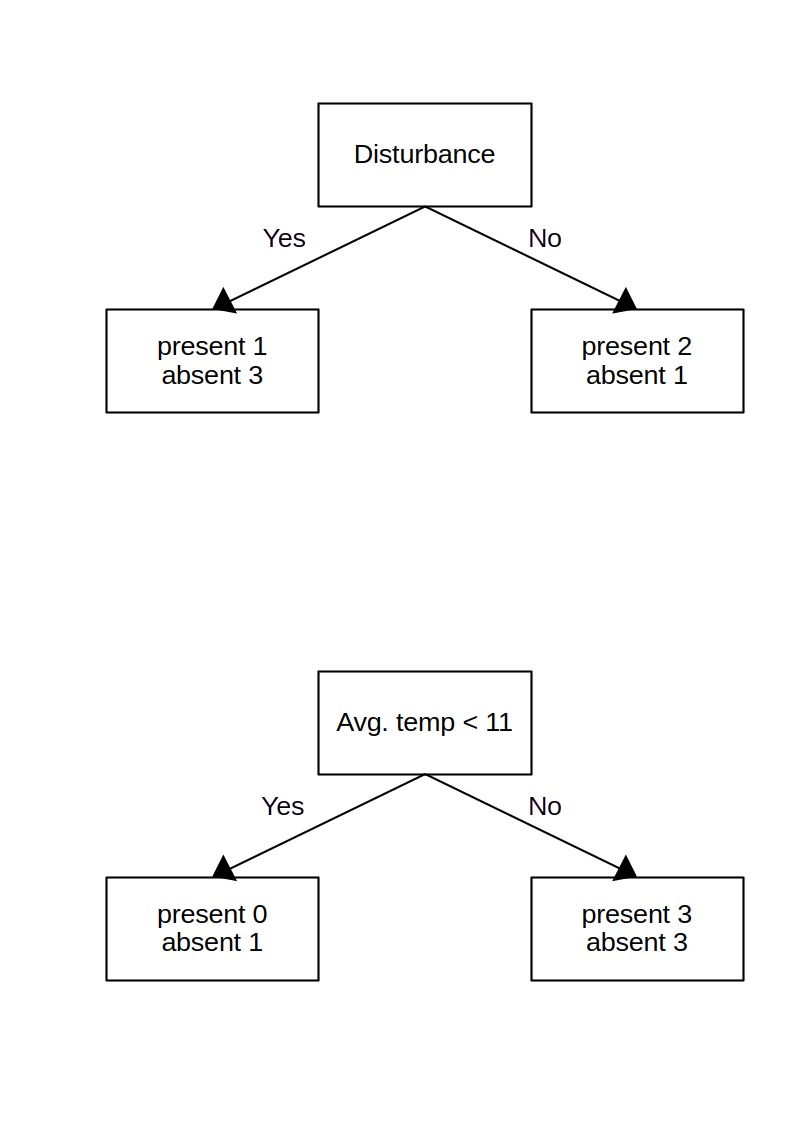
\includegraphics[width=.8\textwidth]{./figs/schemas/gini.png}%
\end{column}
\end{columns}
\end{frame}

\begin{frame}{Gini impurity}
\begin{columns}
    \begin{column}{0.5\textwidth}
\centering
$$
        1 - (\frac{1}{1+3})^2 - (\frac{3}{1+3})^2 = 0.375
 $$
    \end{column}
    \begin{column}{0.5\textwidth}
\centering
    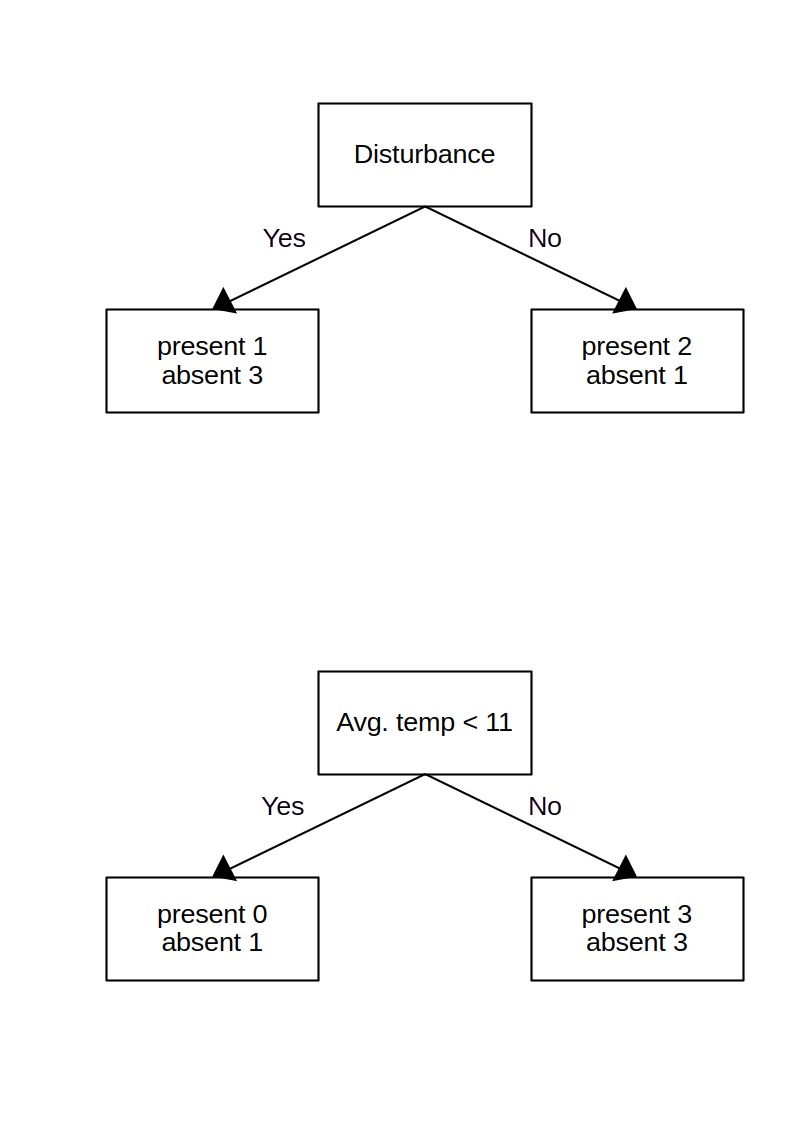
\includegraphics[width=.8\textwidth]{./figs/schemas/gini.png}%
\end{column}
\end{columns}
\end{frame}

\begin{frame}{Gini impurity}
\begin{columns}
    \begin{column}{0.5\textwidth}
\centering
$$
        Leaf~Gini = (\frac{4}{4+3})0.375
 $$
    \end{column}
    \begin{column}{0.5\textwidth}
\centering
    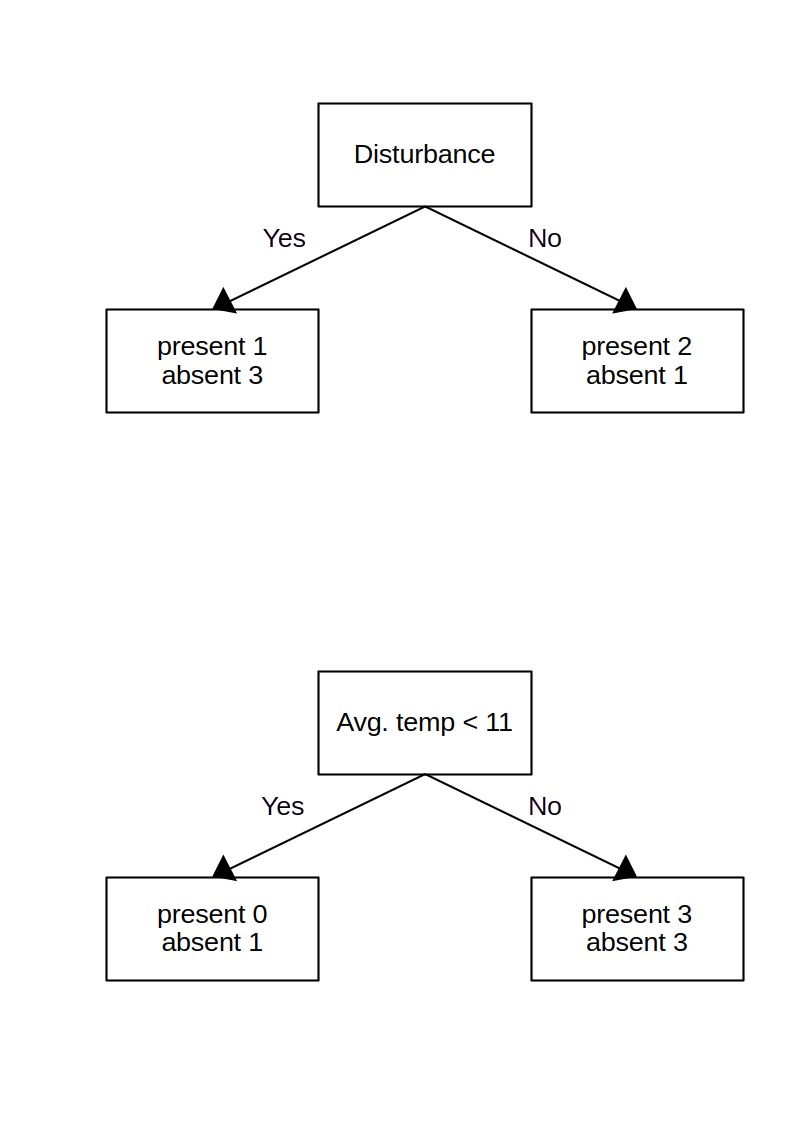
\includegraphics[width=.8\textwidth]{./figs/schemas/gini.png}%
\end{column}
\end{columns}
\end{frame}

\begin{frame}{Gini impurity}
\begin{columns}
    \begin{column}{0.5\textwidth}
\centering
$$
        1 - (\frac{0}{0+1})^2 - (\frac{1}{0+1})^2 = 0
 $$
    \end{column}
    \begin{column}{0.5\textwidth}
\centering
    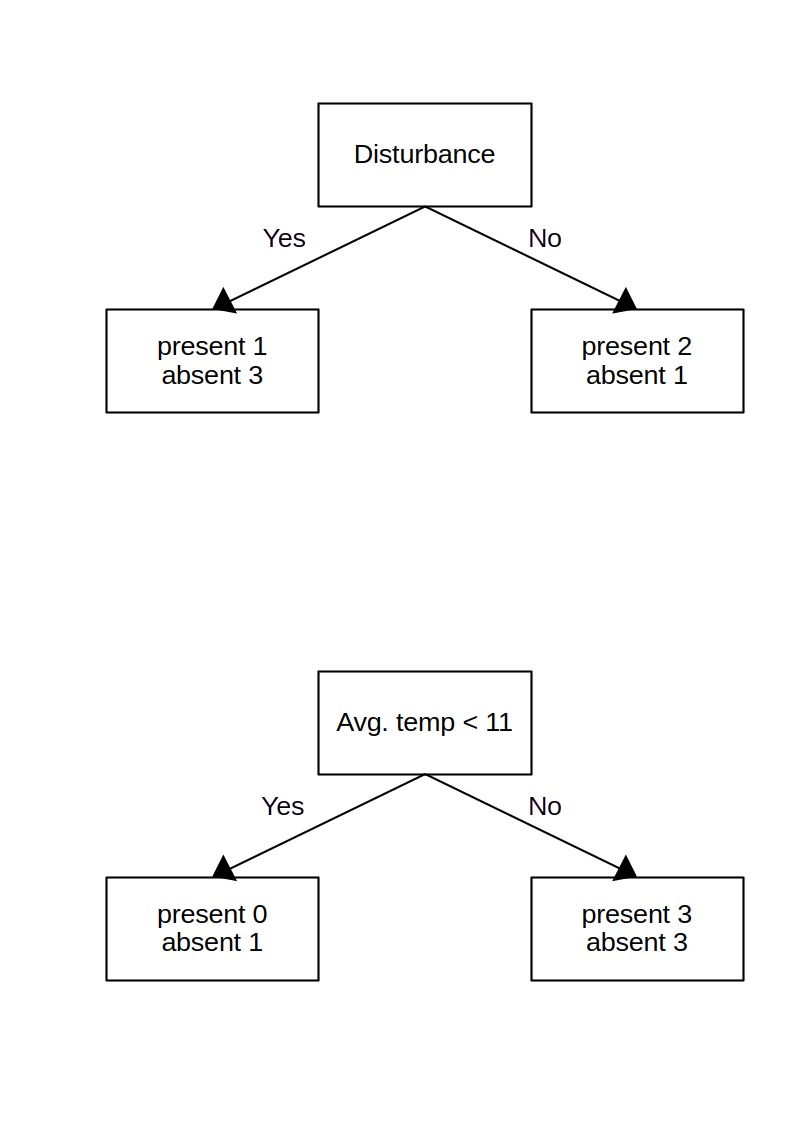
\includegraphics[width=.8\textwidth]{./figs/schemas/gini.png}%
\end{column}
\end{columns}
\end{frame}

\begin{frame}{Building the tree}
\begin{columns}
    \begin{column}{0.5\textwidth}
\centering
{\small
\begin{tabular}{llc|r}
    \toprule
    Disturbance & Habitat & Avg. temp. & Presence \\
    \midrule
    Yes & Shrubs    & 10 & 0 \\
    Yes & Forests   & 12 & 0 \\
    No  & Shrubs    & 18 & 1 \\
    No  & Shrubs    & 25 & 1 \\
    Yes & Shrubs    & 28 & 1 \\
    Yes & Forests   & 30 & 0 \\
    No  & Forests   & 33 & 0 \\
    \bottomrule
\end{tabular}
        }
    \end{column}
    \begin{column}{0.5\textwidth}
\centering
    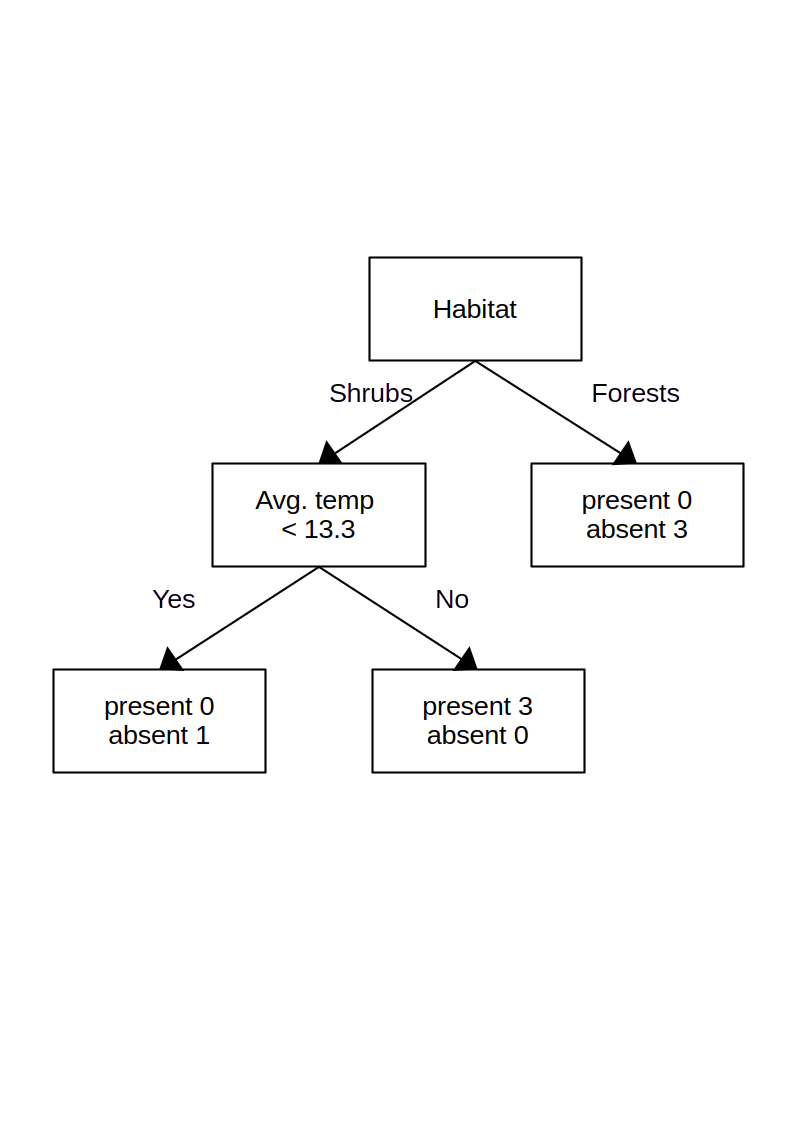
\includegraphics[width=.8\textwidth]{./figs/schemas/tree.png}%
\end{column}
\end{columns}
\end{frame}

\begin{frame}{}
\end{frame}

\section{Random Forests}

\begin{frame}{}
\end{frame}



\begin{frame}{RF advantages and drawbacks}
\begin{columns}
\begin{column}{0.05\textwidth}
\begin{itemize}
    \item[] 
    \item[] 
    \item[] 
    \item[] 
\end{itemize}
\end{column}
    \column{0.45\linewidth}
        \textbf{Advantages}
        \begin{itemize}
            \item<1-> different inputs
            \item<2-> different outputs
            \item<3-> $\approx$ explainable
            \item<4-> pretty fast
            \item<5-> seasonned
        \end{itemize}
    \column{0.45\linewidth}
        \textbf{Drawbacks}
        \begin{itemize}
            \item<6-> need to test hyper-parameters
            \item<7-> \textbf{need for rich descriptors}
            \item[] 
            \item[] 
        \end{itemize}
\end{columns}
\end{frame}

\begin{frame}{Decendants}
    \begin{itemize}
        \item Gradient Boosting
        \item XGBoost
    \end{itemize}
\end{frame}

\begin{frame}{Usefull ressources}
\begin{itemize}
    \item \texttt{scikit-learn} docs !
    \item \href{https://www.youtube.com/@statquest}{StatQuest}
\end{itemize}
\end{frame}

\begin{frame}[plain]
    \Huge{\textbf{Thanks for you attention !}}
    
    \vfill
    
    \LARGE{\textbf{Let's practice !}}
\end{frame}

\appendix
\begin{frame}[allowframebreaks]{References}
\setbeamertemplate{bibliography item}{}
    {\footnotesize \printbibliography[heading=none]}
\end{frame}


\end{document}
